\usetikzlibrary{fit,matrix}
\usetikzlibrary{arrows.meta,calc,shapes}
\providecommand{\computer}{%
    
\includegraphics[width=1cm]{../common/Noun_project_216.pdf}
}
\providecommand{\switch}{%
    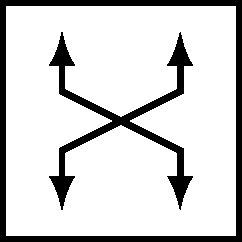
\includegraphics[width=0.9cm]{../common/fig-switch.pdf}
}
\providecommand{\router}{%
    
\includegraphics[width=0.9cm]{../common/fig-router.pdf}
}

\begin{frame}{switch v router: on the wires}
\begin{tikzpicture}
\tikzset{
    computer/.style={inner sep=0mm,outer sep=0mm,execute at begin node={\computer}},
    switch/.style={inner sep=0mm,outer sep=0mm,execute at begin node={\switch}},
    router/.style={inner sep=-1mm,outer sep=0mm,execute at begin node={\router},circle},
    connect/.style={draw,very thick,Latex-Latex},
    connect big/.style={draw,ultra thick,Latex-Latex},
    addr label/.style={align=left,font=\fontsize{9}{10}\selectfont\tt},
}
\node[computer,label={[addr label]south:MAC 00:\ldots:AA\\IP 10.0.1.2},alt=<5>{draw=red,ultra thick,fill=red!10}] (n1-c1) at (0, -2.5) {};
\node[computer,label={[addr label]south:MAC 04:\ldots:BB\\IP 10.0.1.3}]  (n1-c2) at (0, 0) {};
\node[switch] (n1-s1) at (3,-1) {};
\node[switch] (n1-s2) at (5,-4) {};
\node[computer,label={[addr label]south:MAC 05:\ldots:CC\\IP 10.0.1.4}] (n1-c3) at (1, -5) {};
\draw[connect] (n1-c1) -- (n1-s1);
\draw[connect] (n1-c2) -- (n1-s1);
\draw[connect] (n1-c3) -- (n1-s2);
\draw[connect big] (n1-s1) -- (n1-s2);
\node[router,label={[addr label]south:MAC \myemph<5-6>{02:\ldots:DD} / 02:\ldots:DE\\IP: 10.0.1.1 / 10.0.2.15},alt=<5-6>{fill=red!10,draw=red,ultra thick}] (n1n2) at (9, -5) {};
\node[switch] (n2-s1) at (11, -3) {};
\node[computer,label={[addr label]south:MAC 03:\ldots:EE\\IP: \myemph<5>{10.0.2.2}},alt=<5>{draw=red,ultra thick,fill=red!10}] (n2-c1) at (12.5, -4) {};
\draw[connect](n2-s1) -- (n2-c1);

\draw[connect big] (n1-s2) -- (n1n2);
\draw[connect big] (n2-s1) -- (n1n2);
\begin{pgfonlayer}{bg}
    \begin{visibleenv}<2->
        \path[overlay,draw=violet,fill=violet!10]
            (-1.3, -7) -- (5, -7) -- (9, -7) -- (9, -3) -- (4, .75) -- (-1.3, .75) -- cycle;
        \path[overlay,draw=green,fill=green!10]
            (7, 0) -- (8, -2) -- (9, -3) -- (9, -7) -- (13.5, -7) -- (13.5, 0) -- cycle;
        \node[anchor=south,font=\tt] at (5, -7) {10.0.1.0/24};
        \node[anchor=south,font=\tt] at (11, -7) {10.0.2.0/24};
    \end{visibleenv}
\end{pgfonlayer}
\begin{visibleenv}<3->
        \foreach \x [remember=\x as \lastx (initially n1-c1)] in {n1-s1,n1-s2,n1n2,n2-s1,n2-c1} {
            \path[draw,dotted,blue,line width=1mm,arrows=-Latex] (\lastx) -- (\x);
        }
\end{visibleenv}
\begin{visibleenv}<4->
    \path[draw,blue,thick] ($(n1-c1)!0.5!(n1-s1)$) -- (3.7, -1) ++ (0, 1.) coordinate (n1 frame base);
    \node[font=\fontsize{9}{10}\tt,anchor=north west] (n1 outer) at (n1 frame base) {
        00:\ldots:AA\hspace{1mm}$\rightarrow$\myemph<5>{\hspace{1mm}02:\ldots:DD}
    };
    \node[align=left,font=\fontsize{9}{10}\tt,anchor=north west,draw=black!50,very thick,
          alt=<6>{fill=red!10},
    ] (n1 inner) at ([xshift=1mm]n1 outer.south west) {
        10.0.1.3 $\rightarrow$ \myemph<5>{10.0.2.2} \\
        (actual data)
    };
    \path (12, -0) ++ (-2.25, 0.5) coordinate (n2 frame base);
    \node[font=\fontsize{9}{10}\tt,anchor=north west] (n2 outer) at (n2 frame base) {
        02:\ldots:DE\hspace{1mm}$\rightarrow$\hspace{1mm}03:\ldots:EE
    };
    \node[align=left,font=\fontsize{9}{10}\tt,anchor=north west,draw=black!50,very thick,
          alt=<6>{fill=red!10}
    ] (n2 inner) at ([xshift=1mm]n2 outer.south west) {
        10.0.1.3 $\rightarrow$ 10.0.2.2 \\
        (actual data)
    };
\end{visibleenv}
\begin{pgfonlayer}{bg}
    \begin{visibleenv}<4->
    \node[inner sep=0mm,fill=white,draw=blue,very thick,
          fit={(n1 outer) (n1 inner) ([yshift=-1mm]n1 inner.south) ([xshift=1mm]n1 inner.east)}
    ] (n1 box) {};
    \path[draw,blue,thick] ($(n1-s1)!0.5!(n1-s2)$) -- (n1 box);
    \path[draw,blue,thick] ($(n1-s2)!0.5!(n1n2)$) -- (n1 box);
    \node[inner sep=0mm,fill=white,draw=blue,very thick,
          fit={(n2 outer) (n2 inner) ([yshift=-1mm]n2 inner.south) ([xshift=1mm]n2 inner.east)}
    ] (n2 box) {};
    \path[draw,blue,thick] ($(n2-s1)!0.5!(n1n2)$) -- ([xshift=.5cm]n2 box.south west);
    \path[draw,blue,thick] ($(n2-c1)!0.5!(n2-s1)$) -- ([xshift=2cm]n2 box.south west);
    \end{visibleenv}
\end{pgfonlayer}
\begin{visibleenv}<5>
    \node[fill=white,draw=red,ultra thick,align=left] at (3, -5) {
        MAC address = on \textit{local} network \\
        IP address = somewhere else
    };
\end{visibleenv}
\begin{visibleenv}<7>
    \draw[red, ultra thick] (n1 inner) -- (n2 inner)
        node[inner sep=0mm,
             midway,pin={[pin edge={red,ultra thick},fill=white,draw=red,thick,align=center]-90:IP packet copied as is\\placed in new frame}] {};
\end{visibleenv}
% FIXME:    show packets involved
% FIXME:    show frames involved
% FIXME:    show bridge/routing table
\end{tikzpicture}
\end{frame}

\begin{frame}{steps at the sender}
\begin{tikzpicture}
\tikzset{
    computer/.style={inner sep=0mm,outer sep=0mm,execute at begin node={\computer}},
    switch/.style={inner sep=0mm,outer sep=0mm,execute at begin node={\switch}},
    router/.style={inner sep=-1mm,outer sep=0mm,execute at begin node={\router},circle},
    connect/.style={draw,very thick,Latex-Latex},
    connect big/.style={draw,ultra thick,Latex-Latex},
    addr label/.style={align=left,font=\fontsize{9}{10}\selectfont\tt},
}
\node[computer,label={[addr label]south:MAC 00:\ldots:AA\\IP 10.0.1.2},alt=<2->{draw=red,ultra thick,fill=red!10}] (n1-c1) at (0, -2.5) {};
\node[font=\bfseries] at (n1-c1) {src};
\node[computer,label={[addr label]south:MAC 04:\ldots:BB\\IP 10.0.1.3}]  (n1-c2) at (0, 0) {};
\node[switch] (n1-s1) at (3,-1) {};
\node[switch] (n1-s2) at (5,-4) {};
\node[computer,label={[addr label]south:MAC 05:\ldots:CC\\IP 10.0.1.4}] (n1-c3) at (1, -5) {};
\draw[connect] (n1-c1) -- (n1-s1);
\draw[connect] (n1-c2) -- (n1-s1);
\draw[connect] (n1-c3) -- (n1-s2);
\node[router,label={[addr label]south:MAC 02:\ldots:DD / 02:\ldots:DE\\IP: 10.0.1.1 / 10.0.2.15}] (n1n2) at (9, -5) {};
\draw[connect big] (n1-s1) -- (n1-s2);
\draw[connect big] (n1-s2) -- (n1n2);
    \foreach \x [remember=\x as \lastx (initially n1-c1)] in {n1-s1,n1-s2,n1n2} {
        \path[draw,dotted,blue,line width=1mm,arrows=-Latex] (\lastx) -- (\x);
    }

    \path (3.7, -1) ++ (0, 1.) coordinate (n1 frame base);
    \begin{visibleenv}<3>
        \node[font=\fontsize{9}{10}\tt,anchor=north west] (n1 outer pre 1) at (n1 frame base) {
            \myemph<4>{00:\ldots:AA}\hspace{1mm}$\rightarrow$\hspace{1mm}???????
        };
    \end{visibleenv}
    \begin{visibleenv}<4>
        \node[font=\fontsize{9}{10}\tt,anchor=north west] (n1 outer pre 2) at (n1 frame base) {
            \myemph<4>{00:\ldots:AA}\hspace{1mm}$\rightarrow$\hspace{1mm}\myemph<4>{\normalfont 10.0.1.1's MAC}
        };
    \end{visibleenv}
    \begin{visibleenv}<5->
        \node[font=\fontsize{9}{10}\tt,anchor=north west] (n1 outer) at (n1 frame base) {
            00:\ldots:AA\hspace{1mm}$\rightarrow$\hspace{1mm}02:\ldots:DD
        };
    \end{visibleenv}
   \begin{visibleenv}<2->
        \node[
            align=left,font=\fontsize{9}{10}\tt,anchor=north west,draw=black!50,very thick,
            alt=<2>{fill=red!10},
        ] (n1 inner) at ([xshift=1mm]n1 outer.south west) {
            10.0.1.2 $\rightarrow$ \myemph<5>{10.0.2.2}\\
            (actual data)
        };
    \end{visibleenv}
    \begin{visibleenv}<2>
        \path[draw=red,ultra thick,arrows=Latex-](n1 inner.east) -- ++(1cm, 0cm) node[right] {
            packet from upper layer
        };
    \end{visibleenv}
    \begin{visibleenv}<3>
        \path[draw=red,ultra thick,arrows=Latex-,align=left] (n1 outer pre 1.east) -- ++(1cm, 0cm) node[right] {
            need to send at link layer
        };
    \end{visibleenv}
    \begin{visibleenv}<4>
        \path[draw=red,ultra thick,arrows=Latex-,align=left] (n1 outer pre 2.east) -- ++(1cm, 0cm) node[right] {
            routing table says: \\
            to 10.0.1.1 \\
            but need MAC address
        };
    \end{visibleenv}
    \begin{visibleenv}<5>
        \path[draw=red,ultra thick,arrows=Latex-,align=left] (n1 outer pre 1.east) -- ++(1cm, 0cm) node[right] {
            need IP:MAC address table \\
            called neighbor table \\
            or ARP table
        };
    \end{visibleenv}
\begin{pgfonlayer}{bg}
    \begin{visibleenv}<3->
    \node[inner sep=0mm,fill=white,draw=blue,very thick,
          fit={(n1 outer) (n1 inner) ([yshift=-1mm]n1 inner.south) ([xshift=1mm]n1 inner.east)}
    ] (n1 box) {};
    \end{visibleenv}
\end{pgfonlayer}
\tikzset{
    route table/.style={
        matrix of nodes,ampersand replacement=\&,
        nodes={execute at begin node={\strut}},
        column 1/.style={nodes={draw,thin,text width=3cm,font=\fontsize{8}{9}\tt,minimum height=0.4cm,inner sep=.1mm}},
        column 2/.style={nodes={draw,thin,text width=2cm,font=\fontsize{8}{9}\tt,minimum height=0.4cm,inner sep=.1mm}},
        column 3/.style={nodes={draw,thin,text width=1cm,font=\fontsize{8}{9}\tt,minimum height=0.4cm,inner sep=.1mm}},
        row 1/.style={nodes={draw=none,font=\fontsize{8}{9}\selectfont}},
    }
}
%% FIXME: show this with build of IP packet without extra stuff
\begin{pgfonlayer}{fg}
    \begin{visibleenv}<4-5>
    \matrix[
        route table,anchor=north west,
        label={[label distance=0mm,font=\small,alias=route table label]north:src's routing table},
        inner sep=0mm,
        row 3/.style={alt=<4>{nodes={draw=red,fill=red!10}}},
    ] (route table) at (7, -2){
    address \& gateway \& iface \\
    10.0.1.0/24 \& --- \& wired \\
    default \& |[alt=<5>{fill=red!10}]| 10.0.1.1 \& wired \\
    };
    \end{visibleenv}
    \begin{visibleenv}<5->
    \matrix[
        route table,anchor=north west,
        label={[label distance=0mm,font=\small,alias=arp table label]north:src's neighbor table},
        column 1/.style={nodes={draw,thin,text width=2cm,font=\fontsize{8}{9}\tt,minimum height=0.4cm,inner sep=.1mm}},
        column 2/.style={nodes={draw,thin,text width=2cm,font=\fontsize{8}{9}\tt,minimum height=0.4cm,inner sep=.1mm}},
        column 3/.style={nodes={draw,thin,text width=1cm,font=\fontsize{8}{9}\tt,minimum height=0.4cm,inner sep=.1mm}},
        row 3/.style={alt=<4>{nodes={draw=red,fill=red!10}}},
    ] (arp table) at ([yshift=-1cm]route table.south west){
    IP address \& MAC addresss \\
    |[alt=<5>{fill=red!10}]| 10.0.1.1 \& |[alt=<5>{fill=red!10}]| 05:\ldots:DD \\
    10.0.1.4 \& 05:\ldots:CC \\
    };
    \end{visibleenv}
\end{pgfonlayer}
\begin{visibleenv}<4-5>
    \node[fill=white,draw,thick,alt=<4>{ultra thick,draw=red},fit=(route table) (route table label),inner sep=.5mm] {};
\end{visibleenv}
\begin{visibleenv}<5>
    \node[fill=white,draw,thick,alt=<5>{ultra thick,draw=red},fit=(arp table) (arp table label),inner sep=1mm] {};
\end{visibleenv}
% FIXME: show what happens on router
\end{tikzpicture}
\end{frame}

\begin{frame}{steps at the router}
\begin{tikzpicture}
\tikzset{
    computer/.style={inner sep=0mm,outer sep=0mm,execute at begin node={\computer}},
    switch/.style={inner sep=0mm,outer sep=0mm,execute at begin node={\switch}},
    router/.style={inner sep=-1mm,outer sep=0mm,execute at begin node={\router},circle},
    connect/.style={draw,very thick,Latex-Latex},
    connect partial/.style={draw=black!25,overlay},
    connect big/.style={draw,ultra thick,Latex-Latex},
    addr label/.style={align=left,font=\fontsize{9}{10}\selectfont\tt},
}
%\node[computer,label={[addr label]south:MAC 00:\ldots:AA\\IP 10.0.1.2}] (n1-c1) at (0, -2.5) {};
%\node[computer,label={[addr label]south:MAC 04:\ldots:BB\\IP 10.0.1.3}]  (n1-c2) at (0, 0) {};
%\node[switch] (n1-s1) at (3,-1) {};
\node[overlay] (n1-s1) at (3,-1) {};
\node[switch] (n1-s2) at (5,-4) {};
%\node[computer,label={[addr label]south:MAC 05:\ldots:CC\\IP 10.0.1.4}] (n1-c3) at (1, -5) {};
\node[overlay] (n1-c3) at (1, -5) {};
%\draw[connect] (n1-c1) -- (n1-s1);
%\draw[connect] (n1-c2) -- (n1-s1);
\draw[connect,connect partial] (n1-c3) -- (n1-s2);
\draw[connect big,connect partial, ] (n1-s1) -- (n1-s2);
\node[router,label={[addr label]south:MAC {02:\ldots:DD} / 02:\ldots:DE\\IP: 10.0.1.1 / 10.0.2.15}] (n1n2) at (9, -5) {};
\node[font=\bfseries,red] at (n1n2) {rtr}; 
\node[switch] (n2-s1) at (11, -3) {};
%\node[computer,label={[addr label]south:MAC 03:\ldots:EE\\IP: {10.0.2.2}}] (n2-c1) at (12.5, -4) {};
\node[overlay] (n2-c1) at (12.5, -4) {};
\draw[connect,connect partial](n2-s1) -- (n2-c1);

\draw[connect big] (n1-s2) -- (n1n2);
\draw[connect big] (n2-s1) -- (n1n2);
\begin{pgfonlayer}{bg}
    \begin{scope}[overlay]
        \path[overlay,draw=violet,fill=violet!10]
            (-1.3, -7) -- (5, -7) -- (9, -7) -- (9, -3) -- (4, .75) -- (-1.3, .75) -- cycle;
        \path[overlay,draw=green,fill=green!10]
            (7, 0) -- (8, -2) -- (9, -3) -- (9, -7) -- (13.5, -7) -- (13.5, 0) -- cycle;
        \node[anchor=south,font=\tt] at (5, -7) {10.0.1.0/24};
        \node[anchor=south,font=\tt] at (11, -7) {10.0.2.0/24};
    \end{scope}
\end{pgfonlayer}
%        \foreach \x [remember=\x as \lastx (initially n1-s2)] in {n1-s1,n1-s2,n1n2,n2-s1,n2-c1} {
%            \path[draw,dotted,blue,line width=1mm,arrows=-Latex] (\lastx) -- (\x);
%        }
%    \path[draw,blue,thick] ($(n1-c1)!0.5!(n1-s1)$) -- (3.7, -1) ++ (0, 1.) coordinate (n1 frame base);
    \node[font=\fontsize{9}{10}\tt,anchor=north west] (n1 outer) at (n1 frame base) {%
        00:\ldots:AA\hspace{1mm}$\rightarrow${\hspace{1mm}02:\ldots:DD}
    };
    \node[align=left,font=\fontsize{9}{10}\tt,anchor=north west,draw=black!50,very thick,
    ] (n1 inner) at ([xshift=1mm]n1 outer.south west) {%
        10.0.1.3 $\rightarrow$ \myemph<2>{10.0.2.2} \\
        (actual data)
    };
    \path (12, -0) ++ (-2.25, 0.5) coordinate (n2 frame base);
\tikzset{%
    route table/.style={
        matrix of nodes,ampersand replacement=\&,
        nodes={execute at begin node={\strut}},
        column 1/.style={nodes={draw,thin,text width=3cm,font=\fontsize{8}{9}\tt,minimum height=0.4cm,inner sep=.1mm}},
        column 2/.style={nodes={draw,thin,text width=2cm,font=\fontsize{8}{9}\tt,minimum height=0.4cm,inner sep=.1mm}},
        column 3/.style={nodes={draw,thin,text width=1cm,font=\fontsize{8}{9}\tt,minimum height=0.4cm,inner sep=.1mm}},
        row 1/.style={nodes={draw=none,font=\fontsize{8}{9}\selectfont}},
    }
}
    % route and ARP tables
    \begin{pgfonlayer}{fg}
        \begin{visibleenv}<2->
        \matrix[
            fill=white,
            route table,anchor=north west,
            label={[label distance=0mm,font=\small,alias=route table label]north:rtr's routing table},
            inner sep=0mm,
            row 3/.style={alt=<2>{fill=red!10}},
        ] (route table) at (12, -2){
        address \& gateway \& iface \\
        10.0.1.0/24 \& --- \& left \\
        10.0.2.0/24 \& --- \& right \\
        };
        \end{visibleenv}
        \begin{visibleenv}<4->
        \matrix[
            route table,anchor=north,
            label={[label distance=0mm,font=\small,alias=arp table label]north:rtr's neighbor table for right},
            column 1/.style={nodes={draw,thin,text width=2cm,font=\fontsize{8}{9}\tt,minimum height=0.4cm,inner sep=.1mm}},
            column 2/.style={nodes={draw,thin,text width=2cm,font=\fontsize{8}{9}\tt,minimum height=0.4cm,inner sep=.1mm}},
            column 3/.style={nodes={draw,thin,text width=1cm,font=\fontsize{8}{9}\tt,minimum height=0.4cm,inner sep=.1mm}},
            row 3/.style={alt=<4>{nodes={draw=red,fill=red!10}}},
            fill=white,
            inner sep=0mm,
        ] (arp table) at ([yshift=-1cm]route table.south){
        IP address \& MAC addresss \\
        10.0.2.2 \& 03:\ldots:EE \\
        };
        \end{visibleenv}
    \end{pgfonlayer}

    % out going packet
    \begin{visibleenv}<5->
    \node[font=\fontsize{9}{10}\tt,anchor=north west] (n2 outer) at (n2 frame base) {
        02:\ldots:DE\hspace{1mm}$\rightarrow$\hspace{1mm}03:\ldots:EE
    };
    \node[align=left,font=\fontsize{9}{10}\tt,anchor=north west,draw=black!50,very thick,
    ] (n2 inner) at ([xshift=1mm]n2 outer.south west) {
        10.0.1.3 $\rightarrow$ 10.0.2.2 \\
        (actual data)
    };
    \end{visibleenv}
\begin{pgfonlayer}{bg}
    \node[inner sep=0mm,fill=white,draw=blue,very thick,
          fit={(n1 outer) (n1 inner) ([yshift=-1mm]n1 inner.south) ([xshift=1mm]n1 inner.east)}
    ] (n1 box) {};
    %\path[draw,blue,thick] ($(n1-s1)!0.5!(n1-s2)$) -- (n1 box);
    \path[draw,blue,thick] ($(n1-s2)!0.5!(n1n2)$) -- (n1 box);
    \begin{visibleenv}<5->
    \node[inner sep=0mm,fill=white,draw=blue,very thick,
          fit={(n2 outer) (n2 inner) ([yshift=-1mm]n2 inner.south) ([xshift=1mm]n2 inner.east)}
    ] (n2 box) {};
    \path[draw,blue,thick] ($(n2-s1)!0.5!(n1n2)$) -- ([xshift=.5cm]n2 box.south west);
    %\path[draw,blue,thick] ($(n2-c1)!0.5!(n2-s1)$) -- ([xshift=2cm]n2 box.south west);
    \end{visibleenv}
\end{pgfonlayer}
\end{tikzpicture}
\end{frame}


